\documentclass[aps, pre, onecolumn, nofootinbib, notitlepage, groupedaddress, amsfonts, amssymb, amsmath, longbibliography]{revtex4-1}
\usepackage{tabularx}
\usepackage{graphicx}
\usepackage{hyperref}
\usepackage{xcolor}
\hypersetup{
    colorlinks,
    linkcolor={red!50!black},
    citecolor={blue!50!black},
    urlcolor={blue!80!black}
}
\usepackage{bm}
\usepackage{natbib}
\usepackage{longtable}
\LTcapwidth=0.87\textwidth

\newcommand{\Div}[1]{\ensuremath{\nabla\cdot\left( #1\right)}}
\newcommand{\DivU}{\ensuremath{\nabla\cdot\bm{u}}}
\newcommand{\angles}[1]{\ensuremath{\left\langle #1 \right\rangle}}
\newcommand{\KS}[1]{\ensuremath{D_{\text{KS}}(#1)}}
\newcommand{\KSstat}[1]{\ensuremath{\overline{D_\text{KS}(#1)}}}
\newcommand{\grad}{\ensuremath{\nabla}}
\newcommand{\RB}{Rayleigh-B\'{e}nard }
\newcommand{\Reff}{\ensuremath{\text{Re}_{\text{ff}}}}
\newcommand{\Peff}{\ensuremath{\text{Pe}_{\text{ff}}}}


\newcommand\mnras{{MNRAS}}%

\begin{document}
\author{Evan H. Anders}
\affiliation{Dept. Astrophysical \& Planetary Sciences, University of Colorado -- Boulder, Boulder, CO 80309, USA}
\affiliation{Laboratory for Atmospheric and Space Physics, Boulder, CO 80303, USA}
\author{Geoffrey M. Vasil}
\affiliation{University of Sydney School of Mathematics and Statistics, Sydney, NSW 2006, Australia}
\author{Benjamin P. Brown}
\affiliation{Dept. Astrophysical \& Planetary Sciences, University of Colorado -- Boulder, Boulder, CO 80309, USA}
\affiliation{Laboratory for Atmospheric and Space Physics, Boulder, CO 80303, USA}
\author{Lydia Korre}
\affiliation{Laboratory for Atmospheric and Space Physics, Boulder, CO 80303, USA}

\title{Mixed thermal boundary conditions impose an unnecessary thermal rundown on convection simulations}

\begin{abstract}
Astrophysical studies of convection often impose different thermal boundary conditions at the top and the bottom of the domain in an effort to more accurately reflect the natural system being modeled.
In this work, we study \RB convection to show that the use of mixed thermal boundary conditions imposes a long thermal rundown on convective systems which is not experienced by the more classical system where the temperature is fixed at the top and bottom of the domain.
We show that an evolved simulation with mixed thermal boundaries exhibits dynamics whose mean measurements are indistinguishable from a comparable simulation where the temperature is fixed at both boundaries.
We note that thermal relaxation is composed of two parts: changes in the energy reservoir of the system being studied, and changes in the stratification of the system.
Changes in the energy reservoir result from poor choices of initial conditions and boundary conditions, while changes in stratification are the result of interesting convective dynamics.
We warn that measurements made in simulations while the energy reservoir is changing reflect very different dynamics than relaxed simulations.
Finally, we note that the relaxation of these systems effectively amount to a sweep through parameter space, and may be interesting in and of themselves.
\end{abstract}
\maketitle

%%%%%%%%%%%%
%%%%%%%%%%%
% INTRO
%%%%%%%%%%%
%%%%%%%%%%%%

\section{Introduction}

%%%%%%%%%%%%
%%%%%%%%%%%
% EXPERIMENT
%%%%%%%%%%%
%%%%%%%%%%%%

\section{Simulation Details}
\label{sec:simulations}
We study incompressible \RB convection under the same nondimensionalization as we have done previously \cite{anders&all2018}, and including the effects of vertically directed global rotation as in \cite{julien&all1996},
\begin{align}
\Div{\bm{u}} &= 0
	\label{eqn:incompressible}
\\
\frac{\partial \bm{u}}{\partial t} + \left(\bm{\omega} + \frac{1}{\text{Ek }\Reff}\hat{z}\right)\times\bm{u} 
&= - \grad \varpi + T_1\hat{z} - \frac{1}{\Reff}\grad\times\bm{\omega},
	\label{eqn:bouss_momentum}
\\
\frac{\partial T_1}{\partial t}  + \bm{u}\cdot\grad T_1 + w \frac{\partial T_0}{\partial z} 
&= \frac{1}{\Peff}\grad^2 T_1,
	\label{eqn:bouss_energy}
\end{align}
where $\bm{\omega} = \grad \times \bm{u}$ is the vorticity.
The dimensionless control parameters are the Rayleigh, Prandtl, and Ekman numbers,
\begin{equation}
\text{Ra} = \frac{g \alpha L_z^3 \Delta}{\nu\kappa} = \frac{(L_z\,v_{\text{ff}})^2}{\nu\kappa}, \qquad \text{Pr} = \frac{\nu}{\kappa}, \qquad \text{Ek} = \sqrt{\frac{\nu}{2\Omega L_z^2}},
\end{equation}
where $\Delta$ is the dimensionless temperature jump across the domain (described below with our boundary conditions), $\Omega$ is the global rotation frequency, and all other parameters are as described in our previous work \cite{anders&all2018}.
These parameters set the freefall Reynolds and Peclet numbers, $\Reff = \sqrt{\text{Ra}/\text{Pr}}$ and $\Peff = \text{Pr }\Reff$, and throughout this work we hold Pr = 1 so that $\Reff = \Peff$.


In this work, we study two illustrative 3D simulations of rotating convection. 
These simulations employ stress-free, impenetrable upper and lower boundaries,
\begin{equation}
\partial_z u = \partial_z v = w = 0 \, \, \text{at}\,\,z = -0.5, 0.5,
\label{eqn:vel_bcs}
\end{equation}
which are typical of simulations of astrophysical convection \cite{hurlburt&all1984, cattaneo&all1991, korre&all2017}.
We also later include some select two-dimensional simulations for comparison to the \RB convection literature which employ no-slip, impenetrable boundaries,
\begin{equation}
u = w = 0 \, \, \text{at}\,\,z = -0.5, 0.5.
\label{eqn:vel_bcs}
\end{equation}
We study two configurations of thermal boundary conditions: (1) ``mixed'' boundaries where we fix the temperature at the top the flux at the bottom, and (2) fixed-temperature boundaries at the top and the bottom, or:
\begin{equation}
(1): T_1 = 0 \text{ at $z$ = 0.5} \,\&\, \partial_z T_1 = 0 \text{ at $z$ = -0.5};\qquad\qquad
(2): T_1 = 0 \text{ at $z$ = -0.5, 0.5}.
\end{equation}
For case (1), the temperature is nondimensionalized on the initial temperature gradient, $\Delta = L_z \partial_z T_0$, and for case 2 the temperature is nondimensionalized on the initial temperature jump across the domain: $\Delta = \Delta T_0 =  T_0(z=0.5)-T_0(z=-0.5)$.

We utilize the Dedalus\footnote{\url{http://dedalus-project.org/}} pseudospectral framework \cite{burns&all2016} to evolve Eqs.~(\ref{eqn:incompressible}), (\ref{eqn:bouss_momentum}), and (\ref{eqn:bouss_energy}) forward in time.
For our 2D simulations, we use an implicit-explicit (IMEX), third-order, four-stage Runge-Kutta timestepping scheme RK443; for our 3D simulations, we use the second-order, two-stage Runge-Kutta scheme RK222 \cite{ascher&all1997}. 
The code used to run simulations and the code and data used to create the figures in this work are available publicly online in a repository of supplemental materials \cite{anders&all2020a_supp}.
Variables are time-evolved on a dealiased Chebyshev (vertical) and Fourier (horizontal, periodic) domain in which the physical grid dimensions are 3/2 the size of the coefficient grid.  
We study two- (2D) and three-dimensional (3D) convection in which the domain is a cartesian box, whose dimensionless vertical extent is $z \in [-0.5, 0.5]$, and which is horizontally periodic with an extent of $x, y \in [-\Gamma/2, \Gamma/2]$, where $\Gamma = 2$ is the aspect ratio.
In 2D simulations, we set $v = \partial_y = 0$.
For our 2D simulations, we set the aspect ratio to $\Gamma = 2$; for our 3D simulations, we set the aspect ratio to $\Gamma = 10\lambda_c(\text{Ek})$, where $\lambda_c(\text{Ek})$ is the wavelength of convective onset, as has been done by previous authors \cite{stellmach&all2014}.

The initial temperature profile is linearly unstable, $T_0(z) = 0.5 - z$. 
On top of this profile, we fill $T_1$ with random white noise whose magnitude is $10^{-6}/\Peff$, and which is vertically tapered so as to match the thermal boundary conditions.
This ensures that the initial perturbations are much smaller than the evolved convective temperature perturbations, even at large Ra.
We filter this noise spectrum in coefficient space, 
such that only the lower 25\% of the coefficients
have power; this low-pass filter is used to avoid populating the
highest wavenumbers with noise in order to improve the stability of our
spectral timestepping methods.


%%%%%%%%%%%%%%%%%%%%%%%%%%%%%%%%%%%%
%%%%%%%%%%%%%%%%%%%%%%%%%%%%%%%%%%
% Ra & Nu arguments
%%%%%%%%%%%%%%%%%%%%%%%%%%%%%%%%%%
%%%%%%%%%%%%%%%%%%%%%%%%%%%%%%%%%%%%
\subsection{Evolved quantities}
\label{sec:ra_nu_relations}
Throughout this work we will measure and report the evolved value of the Nusselt number.
We define and measure the Nusselt number instantaneously as
\begin{equation}
\text{Nu} \equiv \angles{\frac{w T - \Peff^{-1} \partial_z T}{-\Peff^{-1} \angles{\partial_z T}}}
= 1 + \Peff\frac{\angles{w T}}{-\Delta T},
\end{equation}
where $\angles{}$ represent a volume average ($\angles{A} \equiv \iint A dx dz / \Gamma$ in 2D and $\angles{A} \equiv \iiint A dx dy dz / \Gamma^2$ in 3D for some quantity $A$), and $\Delta T = \angles{\partial_z T}$ is the temperature different between the top and bottom plate.
In the evolved, statistically stationary state, when fixed temperature boundaries are employed, $\text{Nu} = \text{Flux} = 1 + \Peff\angles{wT}$, and when mixed boundaries and a flux nondimensionalization are employed, $\text{Nu} = (\Delta T)^{-1}$.
This suggests that the equilibrated state of a given convective solution is characterized by both a flux and temperature Rayleigh number whose relationship is
\begin{equation}
\text{Ra}_{\partial_z T} = \text{Ra}_{\Delta T} \text{Nu},
\end{equation}
and we will measure both values of Ra as our simulations evolve.

Some additional quantities of interest will be reported throughout this paper.
We will measure the evolved Peclet number of the convective flows in all sections, and in section \ref{sec:rotating_results} we will also report the value of the Rossby number.
We measure these nondimensional quantities instantaneously as
\begin{equation}
\text{Pe} = \angles{|\bm{u}|}\Peff,\qquad \text{Ro} = \angles{|\bm{\omega}|}\text{Ek }\Reff,
\end{equation}
where $|\bm{A}|$ represents the magnitude of the vector $\bm{A}$.





%%%%%%%%%%%%
%%%%%%%%%%%
% RESULTS
%%%%%%%%%%%
%%%%%%%%%%%%
\section{Results}
\label{sec:results}

\subsection{Classical \RB Convection}
\label{sec:2d_results}

\begin{figure}
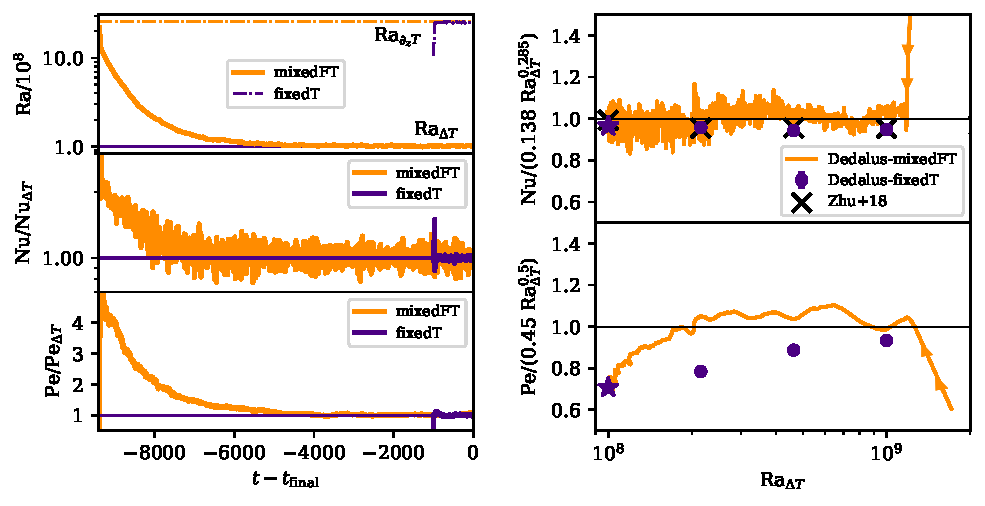
\includegraphics[width=\textwidth]{./figs/rbc_scalar_comparisons.pdf}
\caption{ 
\label{fig:rbc_scalar_comparisons} }
\end{figure}

In the left panels of Fig.~\ref{fig:rbc_scalar_comparisons}, we compare the time evolution of a mixed-FT (green) case to a fixed-T (orange) simulation.
In the top-left panel, we show the evolution of both the temperature and flux Rayleigh numbers of both simulations.
We show the input (flux) Ra of the mixed-FT case and the input (temp) Ra of the fixed-T case as horizontal lines, and overplot the evolution of the Ra$_{\Delta T}$ for the mixed-FT case and the evolution of Ra$_{\partial_z T}$ for the fixed-T case.
While the fixed-T case's flux Ra rapidly latches onto its final value, the mixed-FT case's temp Ra takes thousands of freefall times to equilibrate to its final value.
This fast evolution (fixed-T) and slow evolution (mixed-FT) is also seen in the equilibration of the Nusselt number (middle panel) and Peclet number (bottom panel).

A naive estimate of the thermal evolution timescale of these system is $t_{\text{therm}} = \sqrt{\Peff} = \sqrt{\text{Ra Pr}}$ \cite{anders&all2018}.
For the mixed-FT simulation presented here with Ra = 2.61 $\times 10^9$, this prediction returns $t_{\text{therm}} \approx 5\times 10^{4}$.
**I need to do a derivation and think about this more.

In the upper right panel of Fig.~\ref{fig:rbc_scalar_comparisons}, we show a plot of Nu vs Ra.
The green line shows the path through this space that our mixed-FT simulation traces out.
For reference, we show values of Nu reported for various fixed-T runs from previous work and from our own simulations conducted here.
Remarkably, the mixed-FT case seems to reliably perform a sweep through this parameter space.
However, despite seemingly tracing out the ``proper'' values of Nu(t) vs. Ra(t), the same is not true of the Reynolds number.
In the lower right panel, we plot the trace of Re vs Ra, and see that the mixed-FT case achieves a high value of Re compared to fixed-T cases as it sweeps toward lower values of Ra.
This makes sense; the mixed-FT simulation experiences a vigorous injection of kinetic energy during the convective transient and must slowly wind down from this energized state over time.
These traces through parameter space demonstrate that, unless measurements are taken after convergence is achieved, the dynamics sampled in a mixed-FT case may be misleading.

\begin{figure}
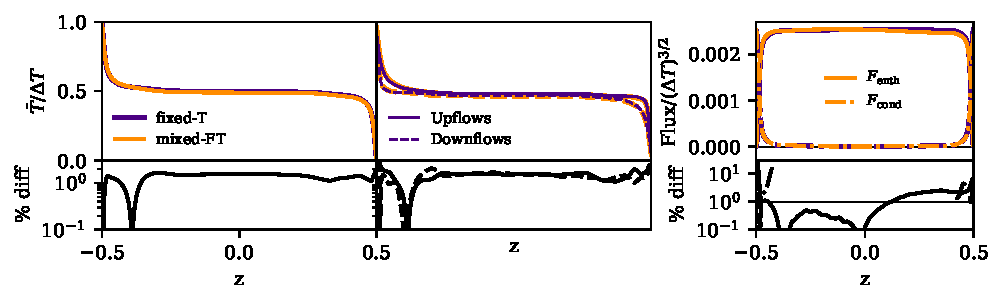
\includegraphics[width=\textwidth]{./figs/rbc_1D_profiles.pdf}
\caption{ 
\label{fig:rbc_1D_profiles} }
\end{figure}

In Fig.~\ref{fig:rbc_1D_profiles}, we compare the horizontally averaged, vertical profiles of our fixed-T and mixed-FT cases.
In the upper left panel, we show the mean temperature profiles achieved in the evolved state of both simulations.
Throughout the full depth, these profiles differ by less than 2\%, as shown in the lower left panel.
In the upper middle panel, we show the mean temperature profile in downflow areas compared to the mean temperature profile achieved in upflow areas.
Surprisingly, despite symmetrical boundary conditiosn in fixed-T simulations and asymmetrical boundary conditions in mixed-FT cases, we find precisely the same asymmetries in upflows/downflows for both sets of boundary conditions.
In general, we find that the boundary layer in upflows is more gradual in hot plumes, and the same is true for downflows and cold plumes.
Once again, these profiles agree to within < 2\%.

In the upper right panel of Fig.~\ref{fig:rbc_1D_profiles}, we plot the system fluxes for both cases.
the fluxes show very good agreement just like the temperature profile.
Throughout the bulk of the domain, the convective enthalpy fluxes agree to within a few \% or less (solid line in bottom right panel).
Due to the conductive fluxes approaching zero in the interior, we cannot measure a \% difference for this flux in the bulk, but we find that it is again within a few percent in the boudnary layers.

\begin{figure}
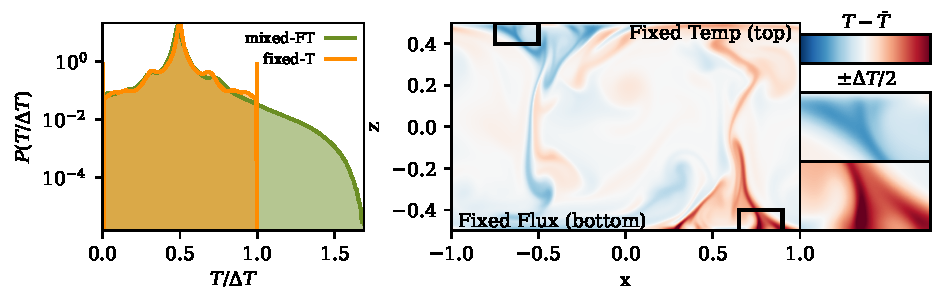
\includegraphics[width=\textwidth]{./figs/rbc_dynamics_asymmetries.pdf}
\caption{ 
\label{fig:rbc_dynamics_asymmetries} }
\end{figure}

In Fig.~\ref{fig:rbc_dynamics_asymmetries}, we examine the dynamical nature of the asymmetries which mixed-FT boundaries introduce into the simulation.
In the left panel, we plot the probability distribution functions of temperature measurements taken throughout the full domain.
These PDFs agree remarkably well for cold temperature (near the shared fixed-T boundary) and through the mean, but diverge for hot temperatures (where the boundary conditions differ).
We find that the mixed-FT pdf has a much longer tail and is capable of achieving much hotter instantaneous temperature values than a fixed-T boundary can.
In order to understand how this is possible, we examine a snapshot of the full temperature field.
In the middle panel, we plot the temperature anomaly -- the temperature field with the mean vertical profile subtracted from it.
We have outlined a portion of a cold plume near the upper (fixed-T) boundary and a portion of a hot plume near the lower (fixed-flux) boundary, and these regions are magnified in the lower right panels.
The fixed-T upper boundary suppresses temperature anomaly at the upper boundary and regulates the temperature minima which can be achieved.
The fixed-flux lower boundary does no such suppression and allows for extreme temperature values to be achieved in the plume-launching area.

\subsection{Fixed-Temp simulations can be used to skip thermal relaxation}

This evidence all suggests that, in a time-averaged, horizontally-averaged, or volume-averaged sense, fixed-T and mixed-FT simulations are 1-to-1 comparable.
However, their dynamics have subtle differences, and it is possible that these differences could be interesting in studies of astrophysical convection (for example, more extreme plume values like those achieved at the fixed-flux plate may interact with a stable layer differently than the more regulated values achieved by a fixed-T plate).
The evolutionary time of mixed-FT cases unfortunately makes running down such simulations in the highly-turbulent, large Rayleigh number regime nearly impossible.
Fortunately, the similarities between these different boundary conditions suggests that the final state of a fixed-temperature simulation, which is rapidly achieved, could serve as an ideal set of initial conditions for a mixed-FT case.

Here's a description of how you scale fixed T  to mixed FT.

In Fig. \ref{fig:Whatever}, we show that indeed this stuff works.

This suggests that thermal relaxation takes place in two parts:
\begin{enumerate}
\item Changes to the experimental energy reservoir,
\item Restratification of the experiment.
\end{enumerate}
The former of these can be skipped through the choice of ``smart'' boundary conditions.
The latter seems to be unimportant in a simple system like the \RB convection studied here.
Takeaway: don't choose boudnary conditiosn where the initial and final energy reservoir are really different.



\subsection{Rotating \RB Convection}
\label{sec:rotating_results}


%\begin{figure}[b]
%\includegraphics[width=\textwidth]{./figs/nu_v_time.png}
%\caption{ \ref{fig:oscillating_plumes}.
%\label{fig:nu_v_time} }
%\end{figure}

%\begin{table}[b!]
%\caption{
%}
%\setlength{\tabcolsep}{12pt}
%\label{table:speed}
%\begin{center}
%\begin{tabularx}{0.72\textwidth}{ c r r c c c }
%\hline																	
%$S$	&	nz$\times$nx$\times$ny	&	$N_{\text{CPU}}$	&	
%$t_{\text{CPU, SE}}$ & $t_{\text{CPU, AE}}$ &$t_{\text{CPU,AE}}/t_{\text{CPU,SE}}$\\
%\hline \hline \multicolumn{6}{c}{\vspace{-0.2cm}}\\
%\multicolumn{6}{c}{\vspace{0.1cm}2D Runs} \\
%\hline
%%2 sig figs, scientific notation, swap SE and AE, right justify Ncpu, 2 sig figs ratio, right justify communicates biggerness. 
%$10^2$	&	64$\times$128	&	32    &  2.2              & 4.4               &     2.0  \\
%$10^3$	&	128$\times$256	&	64    &  53               & 21                &     0.39 \\
%$10^4$	&	256$\times$512	&	128   &  1.2$\times 10^3$ & 1.8$\times 10^2$  &     0.15  \\
%$10^5$	&	512$\times$1024&	256   &  2.4$\times 10^4$ & 2.8$\times 10^3$  &     0.12 \\
%\hline \hline \multicolumn{6}{c}{\vspace{-0.2cm}}\\
%\multicolumn{6}{c}{\vspace{0.1cm}3D Runs} \\
%\hline
%$10^1$	&	32$\times$64$\times$64	    & 512       &   62                 &        1.1$\times 10^2$   & 1.7\\
%$10^2$	&	64$\times$128$\times$128	& 512       &   1.9$\times 10^2$   &        1.1$\times 10^2$   & 0.60 \\
%$10^3$	&	128$\times$256$\times$256	& 2048      &   7.0$\times 10^3$   &        1.4$\times 10^3$   & 0.20 \\
%$10^4$	&	256$\times$512$\times$512	& 8192      &   3.3$\times 10^5$   &        2.3$\times 10^4$   & 0.070\\
%\hline																	
%\end{tabularx}
%\end{center}
%\end{table}



%%%%%%%%%%%%
%%%%%%%%%%%
% CONCLUSION
%%%%%%%%%%%
%%%%%%%%%%%%

\section{Discussion \& Conclusions}
\label{sec:extensions}

\begin{acknowledgments}
EHA acknowledges that this work was supported by NASA Headquarters under the NASA Earth and Space Science Fellowship Program -- Grant 80NSSC18K1199.
This work was additionally supported by NASA LWS grant NNX16AC92G and by the National Science Foundation under grant No.~1616538. 
Computations were conducted with support by the NASA High End Computing (HEC) Program through the NASA  Advanced Supercomputing (NAS) Division at Ames Research Center on Pleiades with allocation GID s1647.
\end{acknowledgments}


\bibliography{biblio.bib}
\end{document}
